% Forward-model schematics, ending at modelled data rather than inference.
% Define \ForegroundWorkflow or \JointWorkflow; otherwise draw only the 21-cm model.
\documentclass[tikz,border=1pt]{standalone}
\usepackage{newtxtext,newtxmath}
\usepackage[T1]{fontenc}
\usepackage{amsmath}
\usetikzlibrary{arrows.meta,calc}
\graphicspath{{plots/}}

% ---------------------------------------------------------------- colours
\definecolor{eorc}{HTML}{1E3A6E}   % 21-cm signal (dark blue)
\definecolor{fgc}{HTML}{A3182F}    % foregrounds (crimson red)
\definecolor{instc}{HTML}{4A5568}  % instrument / data
\definecolor{infc}{HTML}{4A5568}   % inference (same neutral grey as instrument/data)

% ------------------------------------------------------------------ styles
\tikzset{
  panel/.style={draw=#1, fill=white, line width=0.8pt,
                anchor=north west, inner sep=0pt},
  stage/.style={draw=instc, fill=white, line width=0.6pt,
                anchor=north west, inner sep=0pt,
                minimum width=2.91cm, minimum height=2.45cm},
  ttl/.style={font=\footnotesize\bfseries, align=center},
  lbl/.style={font=\footnotesize, align=center},
  small/.style={font=\scriptsize, text=black!70, align=center},
  flow/.style={-{Stealth[length=2.4mm,width=2mm]}, line width=1.1pt, draw=#1},
  flow/.default=instc,
  op/.style={font=\small, text=#1},
  op/.default=black,
  thumb/.style={inner sep=0pt},
}
\newcommand{\bm}[1]{\boldsymbol{#1}}
% \eorcube{x}{y}{size}{file prefix}: cube with front/top/side face images,
% lower-left corner of the front face at (x,y)
\newcommand{\eorcube}[4]{%
  \pgfmathsetmacro{\a}{#3}\pgfmathsetmacro{\dx}{0.38*#3}\pgfmathsetmacro{\dy}{0.265*#3}%
  \begin{scope}[shift={(#1,#2)}]
    \node[thumb, anchor=south west] at (0,0)
         {\includegraphics[width=\a cm,height=\a cm]{#4_front.png}};
    \begin{scope}[cm={1,0,\dx/\a,\dy/\a,(0,\a)}]
      \node[thumb, anchor=south west, transform shape] at (0,0)
           {\includegraphics[width=\a cm,height=\a cm]{#4_top.png}};
    \end{scope}
    \begin{scope}[cm={\dx/\a,\dy/\a,0,1,(\a,0)}]
      \node[thumb, anchor=south west, transform shape] at (0,0)
           {\includegraphics[width=\a cm,height=\a cm]{#4_side.png}};
    \end{scope}
    \draw[white, line width=0.4pt, line join=round]
         (0,0) -- (\a,0) -- (\a,\a) -- (0,\a) -- cycle
         (0,\a) -- (\dx,\a+\dy) -- (\a+\dx,\a+\dy) -- (\a,\a)
         (\a+\dx,\a+\dy) -- (\a+\dx,\dy) -- (\a,0);
  \end{scope}}

\newcommand{\foregroundparameters}[1]{%
  \begin{scope}[xshift=#1cm]
    \node[panel=fgc, fill=fgc!12, minimum width=6.42cm, minimum height=2.45cm] at (0.45,0) {};
    \node[ttl] at (3.66,-0.28) {Image-Domain Foreground Model};
    \node[lbl] at (3.66,-0.62) {$\bm{q}(l,m,n)$};
    \foreach \f/\lab/\k in {fg_q0/q_0/0, fg_q1/q_1/1, fg_q2/q_2/2}{
      \pgfmathsetmacro{\yc}{-1.23-0.36*\k}
      \fill[black, opacity=0.22] (3.68,\yc-0.05) ellipse (1.30 and 0.39);
      \node[thumb] at (3.66,\yc) {\includegraphics[width=2.6cm,height=0.78cm]{\f.png}};
      \node[small, text=black!80, anchor=west] at (5.08,\yc) {$\lab$};
    }
  \end{scope}}
\begin{document}
\begin{tikzpicture}[x=1cm,y=1cm]
\tikzset{grouplabel/.style={fill=white, draw=instc,
  font=\footnotesize\bfseries, inner xsep=3pt, inner ysep=2pt, rotate=90}}

\ifdefined\JointWorkflow
  \def\parametersend{13.97}
\else
  \def\parametersend{6.95}
\fi
\draw[instc, dashed, line width=0.7pt] (0.2,0.08) rectangle (\parametersend,-2.53);
\node[grouplabel] at (0.2,-1.225) {Model Parameters};

\ifdefined\ForegroundWorkflow
  \foregroundparameters{0}
  \def\imagex{0.45}\def\beamx{3.96}\def\visx{7.47}\def\outx{10.98}
  \def\outlineend{10.46}\def\equationx{7.17}
\else
  \node[panel=eorc, fill=eorc!12, minimum width=6.42cm, minimum height=2.45cm] at (0.45,0) {};
  \node[ttl] at (3.66,-0.28) {Fourier-Domain 21-cm Model};
  \node[lbl] at (3.66,-0.62) {$\bm{a}(u,v,\eta)$};
  \eorcube{1.68}{-2.08}{0.55}{eor_k1}
  \eorcube{2.84}{-2.08}{0.76}{eor_k2}
  \eorcube{4.29}{-2.08}{0.98}{eor_k3}
  \node[small, text=eorc] at (1.955,-2.28) {$k_1$};
  \node[small, text=eorc] at (3.22,-2.28) {$k_2$};
  \node[small, text=eorc] at (4.78,-2.28) {$k_3$};
  \def\imagex{3.96}\def\beamx{7.47}\def\visx{10.98}\def\outx{14.54}
  \def\outlineend{13.97}\def\equationx{8.95}
  \node[stage] (fourier) at (0.45,-3.52) {};
  \node[ttl, font=\scriptsize\bfseries] at ($(fourier.north)+(0,-0.25)$) {Sky Fourier Space};
  \node[small, text=black] at ($(fourier.north)+(0,-0.55)$) {$S(u,v,\nu)$};
  \node[thumb] at ($(fourier.north)+(0,-1.55)$) {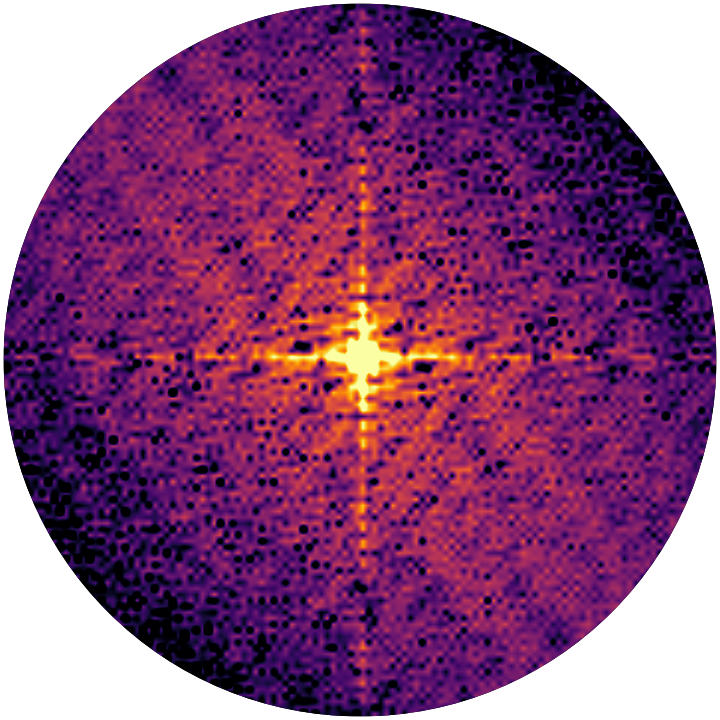
\includegraphics[width=1.6cm]{sky_fourier.png}};
\fi

\ifdefined\JointWorkflow
  \foregroundparameters{7.02}
\fi
\draw[instc, dashed, line width=0.7pt] (0.2,-3.44) rectangle (\outlineend,-6.05);
\node[grouplabel] at (0.2,-4.745) {Forward Model};
\node[stage] (sky) at (\imagex,-3.52) {};
\node[stage] (beam) at (\beamx,-3.52) {};
\node[stage] (vis) at (\visx,-3.52) {};
\foreach \b/\t/\m/\img in {
  sky/{Sky Image Space}/{$I(l,m,\nu,t)$}/sky_image,
  beam/{Primary Beam}/{$P(l,m,\nu)\,I(l,m,\nu,t)$}/sky_beam,
  vis/{Sampled Visibilities}/{$V(\bm{b}_{ij},\nu,t)$}/visibilities}{
  \node[ttl, font=\scriptsize\bfseries] at ($(\b.north)+(0,-0.25)$) {\t};
  \node[small, text=black] at ($(\b.north)+(0,-0.55)$) {\m};
  \node[thumb] at ($(\b.north)+(0,-1.55)$) {\includegraphics[width=1.60cm]{\img.png}};
}
\draw[flow] (sky.east) -- node[above, op] {$\mathbf{P}$} (beam.west);
\draw[flow] (beam.east) -- node[above, op] {$\mathbf{F}^{-1}$} (vis.west);
\ifdefined\ForegroundWorkflow
  \draw[flow=fgc] (1.905,-2.45) -- node[right, op=fgc] {$\mathbf{Q}_z$} (sky.north);
\else
  \draw[flow=eorc] (1.905,-2.45) -- node[right, op=eorc] {$\mathbf{F}_z$} (fourier.north);
  \draw[flow=eorc] (fourier.east) -- node[above, op=eorc] {$\mathbf{F}'$} (sky.west);
\fi
\ifdefined\JointWorkflow
  \draw[flow=fgc] (8.1,-2.45) -- (8.1,-2.97) -- (5.415,-2.97) -- (sky.north);
  \node[op=fgc, anchor=west, inner sep=1pt] at (5.465,-3.20) {$\mathbf{Q}_z$};
\fi

% Retain a single waterfall in place of the likelihood comparison.
\node[stage] (model) at (\outx,-3.52) {};
\node[ttl] at ($(model.north)+(0,-0.25)$) {Modelled Data};
\ifdefined\ForegroundWorkflow
  \node[lbl] at ($(model.north)+(0,-0.60)$) {$\bm{m}_{\rm FG}$};
  \node[font=\small] at (\equationx,-6.43)
    {$\bm{m}_{\rm FG}=\mathbf{T}_{\rm FG}\bm{q}=\mathbf{F}^{-1}\mathbf{P}\mathbf{Q}_z\bm{q}$};
\else
  \ifdefined\JointWorkflow
    \node[lbl] at ($(model.north)+(0,-0.60)$) {$\bm{m}_{21}+\bm{m}_{\rm FG}$};
    \node[font=\small] at (\equationx,-6.43)
      {$\bm{m}=\mathbf{F}^{-1}\mathbf{P}\big(\textcolor{eorc}{\mathbf{F}'\mathbf{F}_z\bm{a}}
      +\textcolor{fgc}{\mathbf{Q}_z\bm{q}}\big)$};
  \else
    \node[lbl] at ($(model.north)+(0,-0.60)$) {$\bm{m}_{21}$};
    \node[font=\small] at (\equationx,-6.43)
      {$\bm{m}_{21}=\mathbf{T}_{21}\bm{a}=\mathbf{F}^{-1}\mathbf{P}\mathbf{F}'\mathbf{F}_z\bm{a}$};
  \fi
\fi
\node[thumb] at ($(model.north)+(0,-1.58)$)
  {
\includegraphics[trim=0 0 1.219cm 0,clip,width=1.65cm]{icon_likelihood.pdf}};
\draw[flow] (vis.east) -- (model.west);
\end{tikzpicture}
\end{document}
